\part{Library resources}
\frame{\partpage}

\begin{frame}{The library}
	\begin{center}
		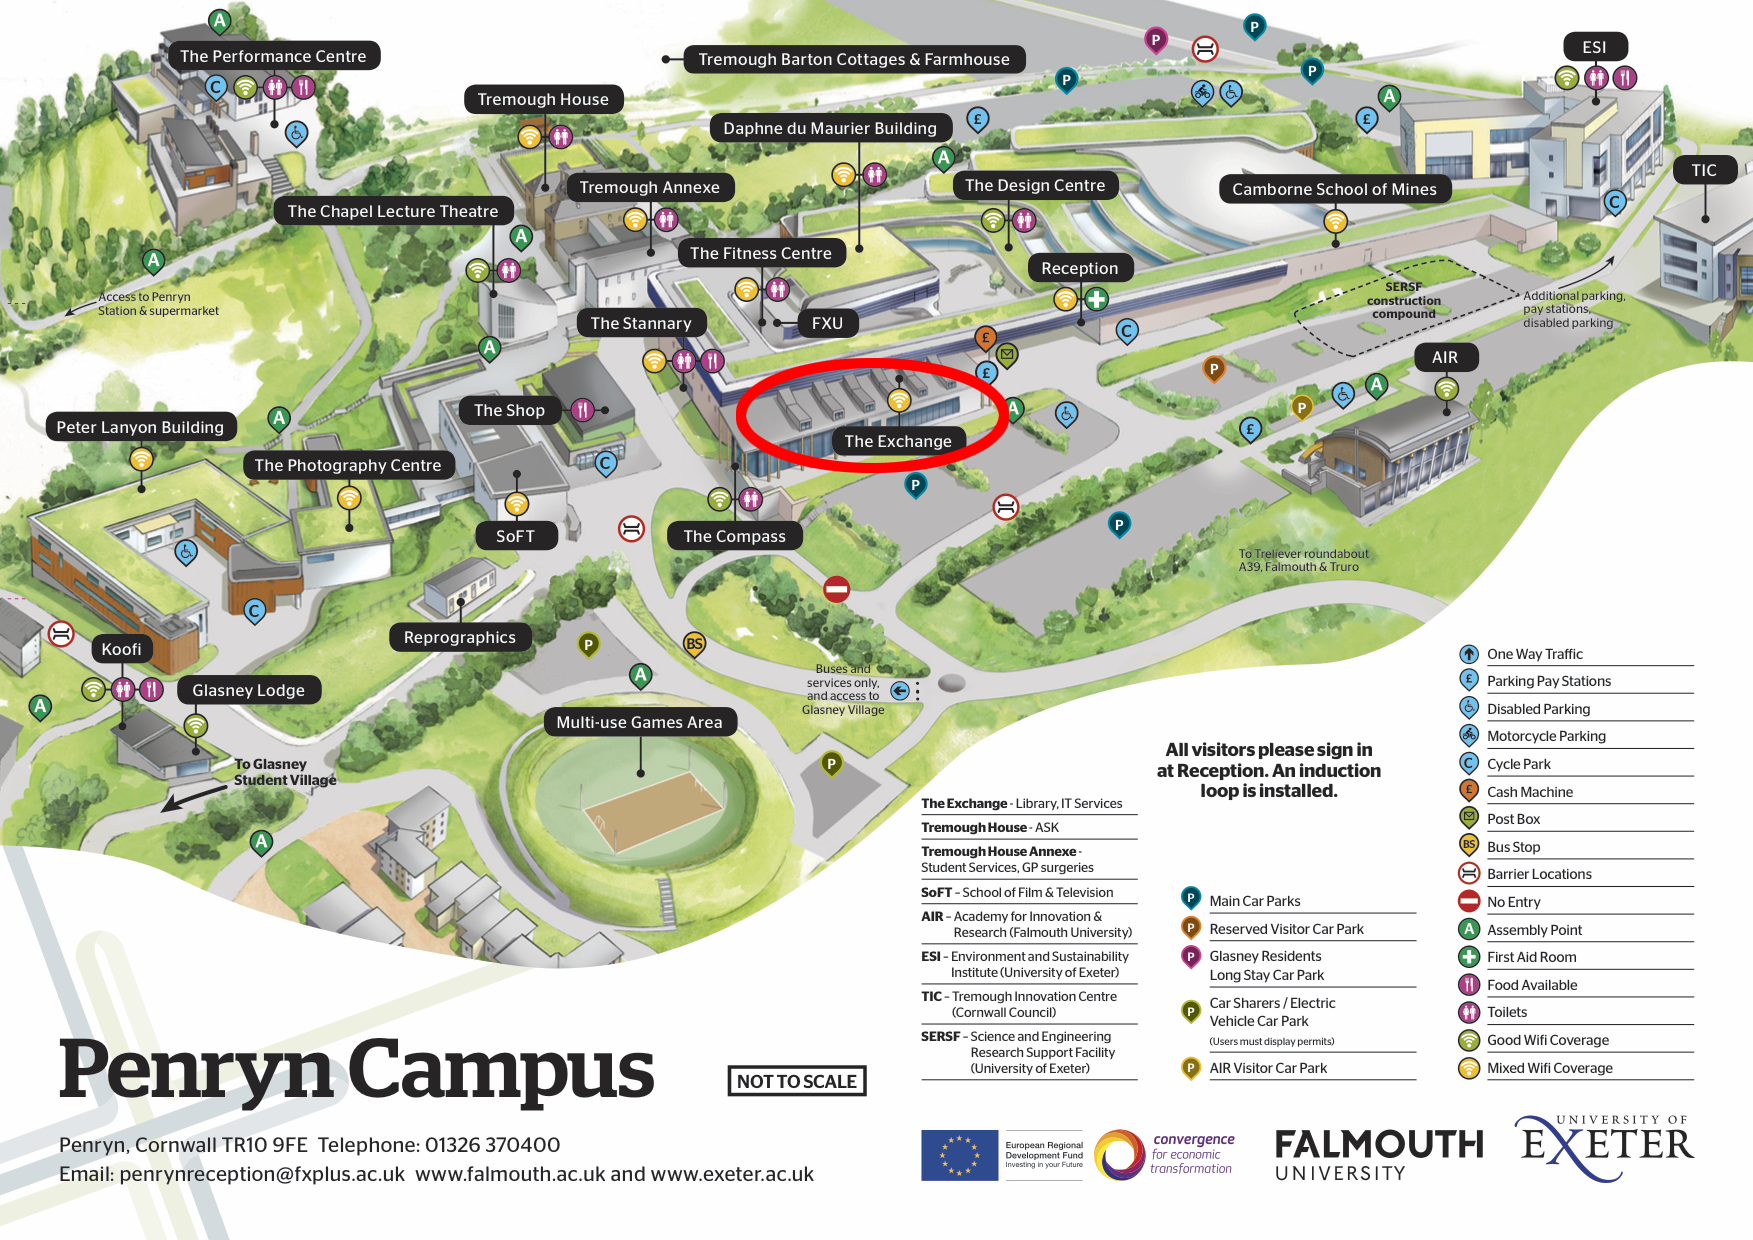
\includegraphics[height=0.7\textheight]{campus_map}
	\end{center}
\end{frame}

\begin{frame}{Library catalogue}
	\begin{center}
		\url{http://library.fxplus.ac.uk/}
	\end{center}
\end{frame}

\begin{frame}{Web proxy}
    \begin{itemize}
        \pause\item Some online resources are only available through the campus network
        \pause\item If not physically on campus, you can access them via \textbf{VPN}
        \pause\item \url{https://webvpn.falmouth.ac.uk/}
        \pause\item Some resources can also be accessed by \textbf{web proxy} through the library website
        \pause\item \url{https://library.fxplus.ac.uk/game-design-computing}
	\end{itemize}
\end{frame}

\begin{frame}{Important resources}
	\begin{itemize}
        \pause\item ACM Digital Library
		\pause\item IEEE Xplore
		\pause\item GDC Vault
	\end{itemize}
\end{frame}

\begin{frame}{How to find papers to read?}
	\begin{itemize}
		\pause\item Specialist databases: ACM Digital Library, IEEE Xplore
		\pause\item Google Scholar
		    \begin{itemize}
		        \pause\item Keyword searches
		        \pause\item Other work by the same author
		        \pause\item Work which has cited papers you have read
		    \end{itemize}
		\pause\item Wikipedia
		    \begin{itemize}
		        \pause\item Not a reliable source itself!
		        \pause\item However most articles have good bibiliographies
		    \end{itemize}
		\pause\item Bibliographies of papers you have read
	\end{itemize}
\end{frame}

\begin{frame}{Finding papers without paying}
	\begin{itemize}
		\pause\item Many papers are \textbf{paywalled}
		\pause\item Little known fact: \textbf{none} of the money from paywalls goes to the authors of the paper!
		\pause\item The university \textbf{subscribes} to ACM and IEEE to give free access to staff and students
		\pause\item Many journals offer free \textbf{open access}
		\pause\item Many authors put papers on their \textbf{personal websites}
		\pause\item Many universities (all UK universities) have \textbf{open access repositories}
			\begin{itemize}
				\pause\item Falmouth: \url{http://repository.falmouth.ac.uk}
			\end{itemize}
		\pause\item Sites like \textbf{sci-hub} have sprung up, providing illegal downloads of papers
	\end{itemize}
\end{frame}
